\def\currentprefix{intro}

\lstset{ %
language=Php,                % the language of the code
basicstyle=\ttfamily,       % the size of the fonts that are used for the code
escapeinside={\%*}{*)},         % if you want to add a comment within your code
morekeywords={*,...},           % if you want to add more keywords to
}


%
%  Introduction
%

%-- Chapter Title
\chapter{Introduction}

Web applications are a fundamental part of our lives and culture. We
use web applications in almost every facet of society: socializing,
banking, health care, taxes, education, news, and entertainment, to
name a few. These web applications are always available from anywhere
with an Internet connection, and they enable us to communicate and
collaborate at a speed that was unthinkable just a few decades ago.

As more and more of our lives and data move to web applications,
hackers have shifted their focus to web applications. In 2011, hackers
stole 1 million usernames and passwords from
Sony~\cite{bilton11:sony}. In 2007, hackers stole 45 million customer
credit cards from TJ Maxx~\cite{jewell07:tjmaxx}. In 2009, hackers
stole 100 million customer credit cards from Heartland Payment
Systems~\cite{acohido09:heartland}. In 2012, hackers stole 24,000
Bitcoins\footnote{These Bitcoins are worth about \$10 million at this
  time of writing.} from BitFloor, a major Bitcoin
exchange~\cite{kirk12:bitfloor}. What all of these instances have in
common is that hackers exploited vulnerabilities in a web application
to steal either usernames and passwords, credit cards, or Bitcoins.

Those same properties that make web applications so attractive to
users also attract hackers. A web application never closes, so they
are always available for hackers. Web applications also house a vast
treasure-trove of data, which hackers can use for monetary gain.
Finally, as we will explore in the next section, web applications are
a complex hodgepodge of various technologies. This complexity,
combined with the intense time-to-market pressure of web applications,
is a breeding ground for bugs and vulnerabilities.

The situation is dire. We must focus on new ways to secure web
applications from attack. We must develop new tools in order to find
the vulnerabilities before a hacker does. We must, because web
applications and the data they store are too important.

\section{History of Web Applications}

The World Wide Web was created by Sir.\ Tim Berners-Lee in 1989 as a
means of sharing information for the CERN research organization. What
began as a means of sharing simple hyper-linked textual documents over
the nascent Internet quickly exploded in popularity over the
proceeding years.

The core of the web has remained relatively the same throughout the
years: a web browser (operated by a user) connects to a web server
using the Hypertext Transfer Protocol (HTTP)~\cite{fielding99:http11}.
The web server then sends back a response, typically in the form of a
HyperText Markup Language (HTML) page~\cite{berjon14:html5}. The web
browser then parses the raw HTML page to create a graphical web page that
is displayed to the user. The fundamental underlying principle, and
the definition of HyperText, is that an HTML page contains links to
\emph{other} HTML pages.

\begin{figure}[tb]
  \centering
  \resizebox{3in}{!}{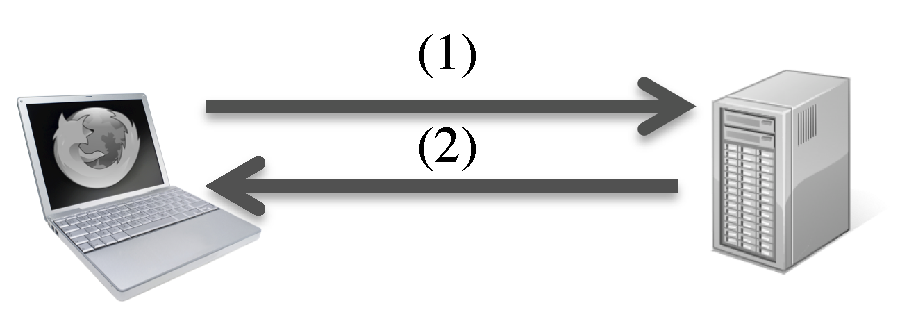
\includegraphics{figures/webserver_interaction_simple.eps}}
  \caption[Example interaction between a web browser and a web
    server.]{Example interaction between a web browser and a web
    server. In (1), the web browser makes an HTTP request to the
    webserver, and in (2) the web server sends the web browser an HTTP
    response containing the HTML of the web page.} 
  \locallabel{webserver-interaction-simple}
\end{figure}


Figure~\localref{webserver-interaction-simple} shows a graphical
representation of the interaction between the web browser and the web
server. In (1), the web browser will make an HTTP request to the web
server, to request a resource. Then, the web server will respond, as
in (2), with an HTTP response which contains the HTML of the requested
web page.

The beginning of the web was envisioned as a set of documents with
links pointing to other documents\footnote{This is where the name
  \emph{web} comes from, as each link forms a strand in the web.}. In
other words, the web was mostly a set of read-only documents (from the
perspective of the user with the web browser). This is where the term
\emph{web site} comes from: a web site is typically thought of as a
collection of documents that exist under the same domain name.

As the web evolved, web sites started to shift from static, read-only
documents. Developers realized that the HTML response returned to the
client could be dynamic---that is, the content of the HTML response
could vary programmatically. This shift in thinking caused web sites to
transition to \emph{web applications} which emulated features of
traditional desktop applications. Web applications enabled scenarios
that caused the web's popularity to increase: e-commerce, news sites, and
web-based email. It is hard to overstate the impact that web
applications had on the uptake of the web. 

Now, with web applications, the architecture of the web changed. When
the web browser makes an HTTP request to the server, instead of
returning a static HTML response, the web server typically will invoke
server-side code. This server-side code is responsible for returning a
response, typically HTML, to the browser. The server-side code can use
any number of inputs to determine the response, but the typically the
server-side code reads the parameters sent in the browser's HTTP
request, consults an SQL database, and returns an HTML response.

\begin{figure}[tb]
  \centering
  \resizebox{5in}{!}{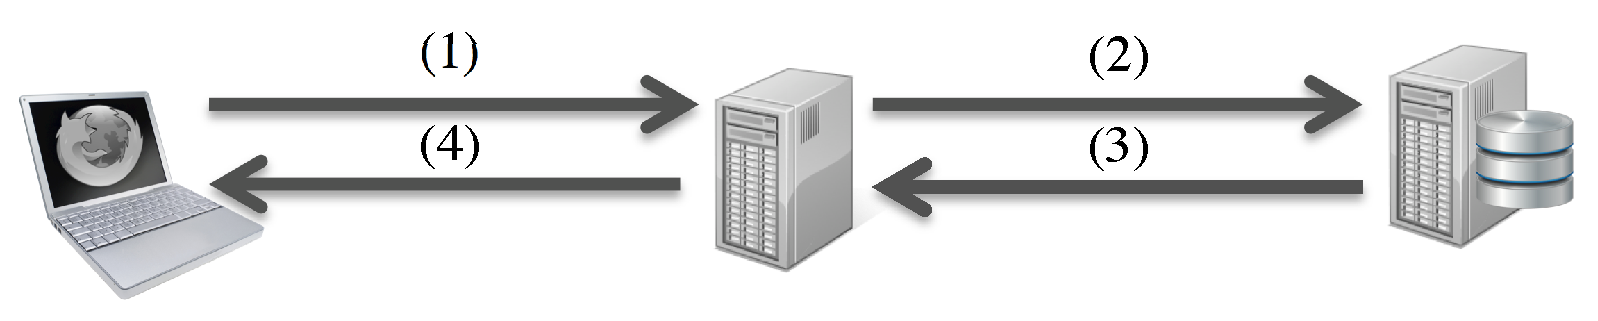
\includegraphics{figures/webserver_interaction_complex.eps}}
  \caption[Sample web application with server-side code and a
    database.]{Sample web application with servers-side code and a
    back-end database. In (1), the web browser makes an HTTP request
    to the web application. Then the server-side code can issue one or
    more SQL queries to the back-end SQL database, shown as (2). The
    SQL server returns the data in (3), which the web application will
    use to generate an HTTP response with HTML, as in (4).}
  \locallabel{webserver-interaction-complex}
\end{figure}


Figure~\localref{webserver-interaction-complex} shows an example web
application with a back-end SQL database. Now, when the web browser
sends an HTTP request to the web application, as in (1), the web
application's server-side code wills start to execute. Then, as (2)
shows, the server-side code can make one or more request to the SQL
database, when executes the queries and returns the data to the
server-side code in (3). Finally, the web application finishes
processing the request and sends an HTTP response with an HTML web
page to the web browser in (4).

The HTTP mechanism is, by design, stateless: Each HTTP request that
the web server receives is, at the beginning, independent of any other
request. It is difficult to build an interactive application on top of
a stateless protocol, thus a standard was developed to add state to
the HTTP process~\cite{kristol97:cookies}. This standard added the
\emph{cookie} mechanism to the HTTP layer. In this way, a web server
can ask the web browser to set a cookie, then, in subsequent requests,
the web browser will include the cookie. Therefore, a web server or
web application can link the requests into a \emph{session} based on
the common cookie and thus develop state-full web applications.

Even after the advent of web applications, the server-side code would
return an HTML page that was statically rendered and displayed to the
user. To change to content on the page or otherwise interact with the
web application, the browser must perform another HTTP request and
response round-trip based on a link the user clicked or a form the
user submitted. In 1997, Brendan Eich, a programmer at Netscape,
created a client-side scripting language called
JavaScript~\cite{ecmascript97}. The user's web browser implemented an
interpreter for this scripting language so that it could manipulate
the web page. Now, with JavaScript, web developers could
programmatically alter the content on the web page without making a
request to the web server. The final linchpin which enabled web
applications to truly rival traditional applications was the creation
and standardization of the XMLHttpRequest JavaScript
API~\cite{vankesteren06:xmlhttprequest}. This API allowed the
client-side JavaScript code to make asynchronous requests to the web
application, and then update the content of the web page according to
the response from the web application. Combined together, these web
application development technologies came to be known as
AJAX~\cite{garrett05:ajax}, which rivaled traditional desktop
applications in functionality. 

This architecture of a web application is what we will use throughout
this chapter to discuss the security aspects of web applications.
Other details and complexities of web applications will be explained
in the chapter where it is needed.

\section{Web Application Vulnerabilities}

The security properties of a web application are similar to the
security of any other software system: confidentially of the data,
integrity of the data, and availability of the application. In this
dissertation, we will focus on attacks that compromise the
confidentially or integrity of the web application's data.

\subsection{Injection Vulnerabilities}

Injection vulnerabilities are to web applications as memory-corruption
vulnerabilities are to binary applications. 

This class of vulnerabilities occur when an attacker is able to
control or influence the value of parameters that are used as part of
an outside\footnote{to the web application's server-side language.}
query, command, or language. If the attacker can manipulate and change
the semantics of the query, command, or language, and this
manipulation compromises the security of the application, then that is
an injection vulnerability.

There are many types of injection vulnerabilities in web applications,
and the types depend on the query, command, or language that is being
injected. These include SQL queries, HTML responses, OS commands,
email headers, HTTP headers, and many more. Next we will focus on two
of the most serious and prevalent classes of injection vulnerabilities
in web applications: SQL injection and Cross-Site Scripting (XSS).

\subsubsection{SQL Injection}

SQL injection vulnerabilities, while declining in the number reported
compared to XSS vulnerabilities, are still numerous and are incredibly
critical when they occur.

The root cause of SQL injection vulnerabilities is that the
server-side code of the web application, to issue an SQL query to the
SQL database, concatenates strings together. This format allows the
queries to be parameterized, and therefore the server-side code can be
more general.

{\ssp
\begin{lstlisting}[language=php, caption={[Example of an SQL injection
        vulnerability.]Example of an SQL injection vulnerability in a
      PHP web application. The attacker-controlled \texttt{\$name} parameter is used
      unsanitized in the SQL query created on Line~2 and issued on Line~3.},
    label=\currentprefix:sql-injection, float,]
$name = $_GET['name'];
$q = "select * from users where name = '" . $name . "';";
$result = mysql_query($q);
\end{lstlisting}
}


The code in Listing~\localref{sql-injection} shows a sample PHP web
application that contains an SQL injection vulnerability. In Line~1 of
this sample, the variable \texttt{\$name} is set based on the value of
the query parameter called \texttt{name}. The \texttt{\$name} variable
is used in Line~2 to construct an SQL query to look up the given user
by name in the SQL table \texttt{users}. The web application issues
the query on Line~3.

The problem is that, according to the server-side language, the
resulting query is simply a string, whereas when that string is passed
to the SQL server, the SQL server parses the string into a SQL query.
Therefore, what the server-side code treats as a simple string is a
complex language with syntax and semantics. 

In Listing~\localref{sql-injection}, the vulnerability comes from the
fact that the query parameter \texttt{name} comes from the user and
therefore may be modified by an attacker. As seen in the example, the
\texttt{\$name} variable is used in the SQL query to select based on
the SQL \texttt{name} column. In order to do this, the programmer
constrains the value to be in between matching
\texttt{\textquotesingle} which is SQL query syntax for delimiting
data. Therefore, for the attacker to alter the semantics of the query,
the attacker need only input something like the following:
\texttt{\textquotesingle or 1=1; \#}. This input would cause the
SQL query that the web application issues to the database to be
the following:

\noindent\lstinline!select * from users where name = '' or 1=1; #';!
\\

The \texttt{\#} is an SQL comment which means that everything after
that in the query is ignored. Now the attacker has been able to alter
the semantics of the SQL query, in this case by adding another SQL
clause (\texttt{or 1=1}) that was not in the original statement.

Thus, in order for an attacker to not alter the semantics of the SQL
query, a web developer must be careful to properly \emph{sanitize} all
potentially attacker-control input. Here sanitize means to transform
the input from the user to a form that renders it neutral for the
target language. In the case of SQL, this typically means converting
any \texttt{\textquotesingle} (which are used by an attacker to escape
out of an SQL query) to the inert
\texttt{\textbackslash\textquotesingle}.

With an SQL injection vulnerability, an attacker can violate both the
confidentially and integrity of the application's data. An attacker
can insert arbitrary data into the database, possibly adding a new
admin user to the web application. Also, an attacker can exfiltrate
any data that the database user can access (typically all data that
the web application can access). Finally, the attacker can also delete
all of the web application's data. These consequences of a single SQL
injection vulnerability are why SQL injection vulnerabilities are so
severe.

To prevent SQL injections with sanitization, a developer must be
extremely careful that no user-supplied data is used in an SQL
statement, including any paths that the data could have taken through
the web application. In practice, this is (understandably) difficult
for developers to always accomplish. Therefore, developers should use
\emph{prepared statements,} which is a way to tell the database the
structure of an SQL query \emph{before} the data is given. In this
way, the database already knows the structure of the SQL query, and
therefore there is no way for an attacker to alter the structure and
semantics of the query. Almost every server-side language or framework
has support for prepared statements. Unfortunately, even with
widespread support for prepared statements, SQL injections are still
frequently found in web applications.

\subsubsection{Cross-Site Scripting}

Cross-Site Scripting (XSS) vulnerabilities are similar in spirit to
SQL injection vulnerabilities. Instead of injection into a SQL
query, XSS vulnerabilities are injections into the HTML output that
the web application generates. XSS vulnerabilities are frequently in
the top three of all reported vulnerabilities in \emph{all} software
systems.

The root cause of XSS vulnerabilities is that the server-side code of
a web application, in order to create the web application's HTML
response, essentially concatenates strings together.

{\ssp
\begin{lstlisting}[language=php, caption={[Example of a XSS 
        vulnerability.]Example of a XSS vulnerability in a
      PHP web application. The attacker-controlled \texttt{\$name} parameter is used
      unsanitized in the HTML output on Line~2.},
    label=\currentprefix:xss-example, float,]
$name = $_GET['name'];
echo "Hello <b>" . $name . "</b>";
\end{lstlisting}
}


Listing~\localref{xss-example} shows an example PHP web application
that has an XSS vulnerability. In Line~1, the variable \texttt{\$name}
is retrieved from the query parameter \texttt{name}. Then,
\texttt{\$name} is used in Line~2 as an argument to PHP's
\texttt{echo} function, which sends its string argument to the HTTP
response. The goal of this code is to output the user's name in bold.
This is accomplished in HTML by wrapping the user's name in a bold tag
(\texttt{<b>}).

If an attacker is able to control the HTML output of the web
application, as the \texttt{\$name} parameter in
Listing~\localref{xss-example}, then the attacker can trick the user's
web browser into executing the attacker's JavaScript. This can be
accomplished in a variety of ways, one example would be inputting the
following for the \texttt{name} query parameter:

\noindent\texttt{<script>alert('xss');</script>}
\\

Matching \texttt{<script>} HTML tags is the way for the web
application to tell the user's browser to execute JavaScript.

The fundamental building block of JavaScript security in the web
browser is the \emph{Same Origin Policy}. In essence, this security
policy means that only JavaScript that comes from the same
origin\footnote{Here, we omit the definition of the same origin. We
  will define it later in the dissertation when necessary.} can
interact. In practice, what this means is that JavaScript running on a
web browser from \texttt{hacker.com} cannot interact with or affect
JavaScript running on the same web browser from \texttt{example.com}.

The name \emph{Cross-Site Scripting} is derived from the fact that XSS
circumvents the browser's Same Origin Policy. By using an XSS
vulnerability, an attacker is able to trick a user's browser to
execute JavaScript code of their choosing in the web application's
origin. This is because, from the browser's perspective, the
JavaScript came from the web application, so the browser happily
executes the attacker's JavaScript along with the web application's
JavaScript.

With an XSS vulnerability, an attacker can compromise a web
application significantly. A popular XSS exploitation technique is to
steal the web application's cookies and send them to the attacker.
Typically the web application's cookies are used to authenticate and
keep state with the web application, which could allow the attacker to
impersonate the user.

By executing JavaScript in the same origin as the web application, the
attacker's JavaScript has total control over the graphical appearance
of the web page. What this means is that the attacker can completely
alter the look of the web page, and could, for instance, force the
page to resemble the web application's login form. However, once the
user puts their information into the form, the attacker's JavaScript
could steal that information. In this way, the attacker is able to
phish the user's credentials, except in this instance the user is on
the proper domain name for the web application.

Another insidious thing that an attacker's JavaScript can do if it
executes in the user's browser is interact with the web application on
behalf of the user\footnote{This defeats any CSRF protection that the
  web application has enabled, as the attacker's JavaScript can read
  the web application's CSRF tokens.}. In practice, what this means is
that the attacker's JavaScript can interact with the web application,
and the web application has no way of knowing that the requests did
not come from the user. Imagine an attacker's JavaScript sending
emails on a user's behalf or initiating a bank transfer.

XSS vulnerabilities can be fixed by proper sanitizaiton at all program
points in the web application that output HTML. This sanitization
process typically will convert entities that are significant in
parsing HTML to their display equivalent. For instance, the HTML
\texttt{<} character is transfer to its HTML entity equivalent
\texttt{\&gt;}, which means to display a \texttt{<} character on the
resulting web page, rather than starting an HTML tag.

There are a number of practical difficulties that make properly
sanitizing output for XSS vulnerabilities particularly challenging
(especially when compared to SQL injection vulnerabilities). One
difficulty is that, as shown by Saxena, Molnar, and
Livshits~\cite{saxena11:scriptgard}, there are numerous types of
sanitization for XSS vulnerabilities, and which type of sanitization
to use depends on \emph{where} the output is used in the resulting
HTML page. This means that the developer must reason not only about
all program paths that a variable may take to get to a specific
program point (to see if an attacker can influence its value), but
also about all the different places in the HTML output where the
variable is used. The complex nature of XSS vulnerabilities contribute
to the reason that it is still the most frequent web application
vulnerability.

Unfortunately XSS vulnerabilities have no easy, widely supported fix,
as prepared statements are to SQL injection vulnerabilities. However,
in Chapter~\ref{dedacota} we will look at an approach to fundamentally
solve a large class of XSS vulnerabilities.

\subsection{Logic Flaws}

Logic flaws are a class of vulnerabilities that occur when the
implemented logic of the web application does not match with the
developer's intended logic of the web application. One popular example
would be, on an ecommerce application, if a user is able to submit a
coupon multiple times, until the price of the item is zero. Another
example might be a financial services web application which
accidentally sends confidential financial reports to unauthorized
users. 

An injection vulnerability can affect any web application, and the fix
of the vulnerability will be the same, regardless of the underlying
web application. In contrast, logic flaws are specific and unique to
the web application. Identical behavior that appears in two web
applications may be a logic flaw in one but a security vulnerability
in the other. Consider the behavior of an unauthenticated user
altering the content of a web page. In most applications, this would
represent a vulnerability, however it is the core mechanic and
defining feature of a wiki, such as Wikipedia. The distinguishing
feature of logic flaw vulnerabilities is that the web application code
is functioning correctly---that is, an attacker is not able to alter
how the code executes or execute code of her choosing, however the
behavior that the code executes violates the developer's security
model of the application. Therefore, these vulnerabilities are
incredibly difficult to detect in an automated fashion, as the
automated tool must reverse engineer the developer's intended security
model.

In Chapter~\ref{fear-the-ear}, we will describe a novel class of logic
flaw vulnerabilities called Execution After Redirect.

\section{Securing Web Applications}

Given their rise in popularity, ensuring that web applications are
secure is critical. Security flaws in a web application can allow an
attacker unprecedented access to secret and sensitive data. 

There are numerous approaches to secure web applications, depending on
where one wants to focus. One approach is to detect attacks as they
happen and block the attack traffic. Another approach is to construct
the web application in a way such that it is not vulnerable to entire
classes of security vulnerabilities. Finally, and the approach taken
in the majority of this dissertation, is automated tools to
automatically find vulnerabilities in web applications.


\subsection{Anomaly Detection}

One way to secure web applications is to have tools and approaches
that look for attacks against web applications in the inbound web
traffic~\cite{robertson09:dissertation}. There are many approaches in
this area, but most of them involve first creating a model of the
normal behavior of the web application. Then, after this model is
created, a monitoring/detection phase starts which analyzes inbound
web application traffic looking for anomalous web requests which signify
an attack. Depending on the anomaly detection system, the request can
be blocked or prevented at that time.

Anomaly detection systems are good for preventing unknown exploits
against the web application. However, the effectiveness of the anomaly
detection depends on the creation of the web application model and the
presence of extensive attack-free traffic. In practice, it is
difficult to automatically create extensive attack-free traffic.

Modern web application can use anomaly detection systems in production
environments as a defense-in-depth approach.

%% \subsection{Secure Construction}

%% Another approach to secure web applications is to create them in such
%% a way as 

\subsection{Vulnerability Analysis Tools}

Vulnerability analysis is the art of finding vulnerabilities in
software. The idea is to find vulnerabilities either before an
application is deployed or before an attacker is able to find the
vulnerability.

Manual vulnerability analysis is when a team of humans manually
analyze an application for vulnerabilities. These manual vulnerability
analyses, frequently called \emph{pentesting,} employ a team of
experts to find vulnerabilities in a software system. The downside is
that an expert's time is costly, and therefore, due to the cost, a
company will very infrequently do an external pentest of its
web applications.

Vulnerability analysis tools are automated approaches to find
vulnerabilities in software. The goal of this type of software is to
find all possible vulnerabilities in an application. The core idea is
to develop software that can encapsulate a human security expert's
knowledge.

Because vulnerability analysis tools are automated, they can be used
against a variety of applications. Furthermore, they are significantly
less expensive than hiring a team of human experts, so they can be
used much more frequently throughout the software development process.

Vulnerability analysis tools can be categorized based on what
information of the web application they use. In the following sections
we will describe the difference between white-box, black-box, and
grey-box vulnerability analysis tools.

\subsubsection{White-Box}

A white-box vulnerability analysis tool looks at the source code of
the web application to find vulnerabilities. By analyzing the source
code of the web application, a white-box tool can see \emph{all}
potential program paths throughout the application. This enables a
white-box tool to potentially find vulnerabilities along all program
paths. Typically approaches leverage ideas and techniques from the
program analysis and static analysis communities to find
vulnerabilities.

The biggest strength of white-box tools is that they are able to see
all possible program paths through the application. However, as
precisely identifying all vulnerabilities in an application via static
analysis is equivalent to the halting problem, trade-offs must be made
in order to create useful tools. The trade-off that is often made in
white-box tools is one of being sound rather than complete. What this
means is that a white-box tool will report vulnerabilities that are
not actual vulnerabilities. This is usually because the static
analysis will over-approximate the program paths that the application
can take. Thus, there will be vulnerabilities reported that cannot
occur in practice.

The downside of white-box tools is that they are tied to the specific
language or framework. A white-box vulnerability analysis tool written
for PHP will not work for Ruby on Rails without significant
engineering work. These tools are tightly coupled to not only language
features, but also framework features. 

\subsubsection{Black-Box}

In contrast to white-box tools, black-box vulnerability analysis tools
assume no knowledge of the source-code of the web application. Instead
of using the source code, black-box tools interact with the web
application being tested just as a user with a web browser would.
Specifically, this means that the black-box tools issue HTTP requests
to the web application and receive HTTP responses containing HTML.
These HTML pages tell the black-box tool how to generate new HTTP
requests to the application.

Black-box tools first will crawl the web application looking for all
possible \emph{injection vectors} into the web application. An
injection vector is any way that an attacker can feed input into the
web application. In practice, web application injection vectors are:
URL parameters, HTML form parameters, HTTP cookies, HTTP headers, URL
path, and so on.

Once the black-box tool has enumerated all possible injection vectors
in the application, the next step is to give the web application input
which is intended to trigger or expose a vulnerability in the web
application. This process is typically called \emph{fuzzing.} The
specifics of choosing which injection vectors to fuzz and when are
specific to each black-box tool. 

Finally, the black-box tool will analyze the HTML and HTTP response to
the fuzzing attempts in order to tell if the attempt was successful.
If it was, the black-box tool will report it as a vulnerability.

There are two major benefits of black-box tools as opposed to
white-box tools. The first is that black-box tools are general and can
find vulnerabilities in \emph{any} web application, regardless of what
language the server-side code is written in. In this way, black-box
tools emulate an external hacker who has no access to the source code
of the application. Therefore, black-box tools are applicable to a
much larger number of web applications. 

The second major benefit is that black-box tools have significantly
lower false positives\footnote{A \emph{false positive} is a
  vulnerability that the tool reports which is not actually a
  vulnerability.} than white-box tools. This is because the fuzzing
attempt actually tries to trigger the vulnerability, and, for most web
vulnerabilities, a successful exploitation will be evident in the
resulting HTML page. Ultimately, lower false positives causes the
developers who run these tools against their own web applications to
trust the output of a black-box tool over a white-box tool.

The drawback of a black-box tool is that it is not guaranteed to find
all vulnerabilities in your web application. This limitation is
because a black-box tool can only find vulnerabilities along program
paths that it executes, whereas a white-box tool can see all program
paths through an application.

\subsubsection{Grey-Box}

As the name suggests, grey-box tools are a combination of white-box
techniques and black-box techniques. The main idea is to use white-box
static analysis techniques to generate possible vulnerabilities. Then,
there is a confirmation step where the tool will actually try to
exploit the vulnerability. Only if this step is successful will the
tool report the vulnerability.

Grey-box tools inherit the benefits of white-box tools: The ability to
find vulnerabilities in all program paths along with the low false
positive rate associated with black-box tools (as the vulnerabilities
are verified by the black-box techniques). However, grey-box tools also
inherit the drawbacks of white-box tools: Applicability to a single web
application language or framework. Therefore, these types of tools are
not as popular as white-box and black-box tools. 
\\

\noindent{}Given the empowering nature of web applications, it is
clear that securing web applications is important.
Specifically, we must focus on the needs of the users: making sure
that their data is safe, and that they are safe while browsing the
web. To accomplish this, I believe that we must make the necessary
strides to create automated tools that are able to automatically find
security vulnerabilities. These tools can be used by developers with
no security expertise, thus putting developers on a level playing
field with the attackers.
\\

\noindent{}In this dissertation, I make the following contributions to securing
web applications from attack:

\begin{itemize}

\item I first methodically analyze existing black-box web application
  vulnerability scanners. We develop a known-vulnerable web
  application, then evaluate several real-world black-box web
  application vulnerability scanners to identify their strengths and
  weaknesses.

\item Then, using the previously developed work as a guide, I aim to
  solve the biggest problem restricting modern black-box web
  application vulnerability scanners: They do not understand that they
  are analyzing a web \emph{application} with state. I develop an
  approach to automatically reverse-engineer the state machine of a
  web application solely through black-box interactions. Incorporating
  this knowledge into a black-box web application vulnerability
  scanner enables the scanner to test significantly more of the web
  application.

\item I identify and study a novel class of web application
  vulnerabilities, called Execution After Redirect, or EARs. These
  logic flaw vulnerabilities can affect web applications written in a
  number of languages or frameworks. In addition to studying this
  class of vulnerabilities, we developed a white-box static analysis
  tool to automatically identify EARs in Ruby on Rails web
  applications. By applying this tool to a large corpus of real-world
  open-source web application, we found many previously unknown
  vulnerabilities.

\item Finally, I propose a new approach to fundamentally solve
  Cross-Site Scripting vulnerabilities. By using the fundamental
  security principles of Code and Data separation, we can view XSS
  vulnerabilities as a problem of Code and Data separation. New
  applications can be designed with Code and Data separation in mind,
  however it is difficult to separate Code and Data manually. To
  prevent XSS vulnerabilities in existing web applications, I created
  a tool to automatically perform Code and Data separation for legacy
  web applications. After applying this tool, the web applications are
  fundamentally secure from server-side XSS vulnerabilities.

\end{itemize}

% Thesis Statement
% --------------------------------------------------------------------
%% \pagebreak
%% \section*{Thesis Statement}

%% Is this something I need? Did wkr have it?



